\documentclass[
10pt, % Set the default font size, options include: 8pt, 9pt, 10pt, 11pt, 12pt, 14pt, 17pt, 20pt
%t, % Uncomment to vertically align all slide content to the top of the slide, rather than the default centered
aspectratio=169, % Uncomment to set the aspect ratio to a 16:9 ratio which matches the aspect ratio of 1080p and 4K screens and projectors
]{beamer}

\usepackage[all]{xy}

\usepackage[spanish]{babel}
\usepackage[utf8]{inputenc}

\graphicspath{{Images/}{./}} % Specifies where to look for included images (trailing slash required)

\usepackage{booktabs} % Allows the use of \toprule, \midrule and \bottomrule for better rules in tables

%\usepackage{tikz}
%\usetikzlibrary{positioning}
%\usetikzlibrary{shapes,arrows,arrows,positioning,fit}

\usepackage{tikz}
\usepackage{adjustbox}
\usetikzlibrary{arrows, shapes}

\usepackage{forest}

\usepackage{multirow}

\usepackage{graphicx}
\usepackage{hyperref}

\usepackage{xcolor,listings}
\usepackage{textcomp}
%\usepackage{color}

\usepackage{enumitem}

\usepackage{xcolor}

\usepackage{verbatim}
\usepackage{changepage}

\usepackage{algpseudocode}
\usepackage{gensymb}

\usepackage{venndiagram}

\usepackage{graphicx}

\usepackage{array}

\usepackage{colortbl}
\usetikzlibrary{positioning}

% \usepackage{media9}

% \usepackage{algorithm}
% \usepackage{algorithmic}

\providecommand{\abs}[1]{\lvert#1\rvert}

%----------------------------------------------------------------------------------------
%	SELECT LAYOUT THEME
%----------------------------------------------------------------------------------------
\usetheme{Madrid} 

%----------------------------------------------------------------------------------------
%	SELECT COLOR THEME
%----------------------------------------------------------------------------------------
%\usecolortheme{beaver}
%\usecolortheme{seahorse}
\usecolortheme{spruce} % verde suave
%\usecolortheme{whale}
%\usecolortheme{wolverine}

%----------------------------------------------------------------------------------------
%	SELECT FONT THEME & FONTS
%----------------------------------------------------------------------------------------
\usefonttheme{default} % Typeset using the default sans serif font
%\usefonttheme{serif} % Typeset using the default serif font (make sure a sans font isn't being set as the default font if you use this option!)
%\usefonttheme{structurebold} % Typeset important structure text (titles, headlines, footlines, sidebar, etc) in bold
%\usefonttheme{structureitalicserif} % Typeset important structure text (titles, headlines, footlines, sidebar, etc) in italic serif
%\usefonttheme{structuresmallcapsserif} % Typeset important structure text (titles, headlines, footlines, sidebar, etc) in small caps serif

%------------------------------------------------

%\usepackage{mathptmx} % Use the Times font for serif text
%\usepackage{palatino} % Use the Palatino font for serif text

\usepackage{helvet} % Use the Helvetica font for sans serif text
%\usepackage[default]{opensans} % Use the Open Sans font for sans serif text
%\usepackage[default]{FiraSans} % Use the Fira Sans font for sans serif text
\usepackage[default]{lato} % Use the Lato font for sans serif text

%----------------------------------------------------------------------------------------
%	SELECT INNER THEME
%----------------------------------------------------------------------------------------
\useinnertheme{circles}


\setbeamertemplate{footline} % Uncomment this line to remove the footer line in all slides
%\setbeamertemplate{footline}[page number] % Uncomment this line to replace the footer line in all slides with a simple slide count

\setbeamertemplate{navigation symbols}{} % Uncomment this line to remove the navigation symbols from the bottom of all slides

%----------------------------------------------------------------------------------------
%	PRESENTATION INFORMATION
%----------------------------------------------------------------------------------------

\title[Short Title]{Ranking y posicionamiento en la Web} 

\subtitle{Sistemas de Recuperación de Información}

\author{Lic. Carlos León González \\ Dra.C. Lucina García Hernández}

\institute[UC]{Facultad de Matem\'atica y Computaci\'on \\ Universidad de La Habana \\ \smallskip }

\date{1 de julio de  2024} % Presentation date or conference/meeting name, the optional parameter can contain a shortened version to appear on the bottom of every slide, while the required parameter value is output to the title slide

%----------------------------------------------------------------------------------------

\begin{document}
	
	\lstset{
		literate=%
		{á}{{\'a}}1
		{í}{{\'i}}1
		{é}{{\'e}}1
		{ý}{{\'y}}1
		{ú}{{\'u}}1
		{ó}{{\'o}}1
		{ě}{{\v{e}}}1
		{š}{{\v{s}}}1
		{č}{{\v{c}}}1
		{ř}{{\v{r}}}1
		{ž}{{\v{z}}}1
		{ď}{{\v{d}}}1
		{ť}{{\v{t}}}1
		{ň}{{\v{n}}}1                
		{ů}{{\r{u}}}1
		{Á}{{\'A}}1
		{Í}{{\'I}}1
		{É}{{\'E}}1
		{Ý}{{\'Y}}1
		{Ú}{{\'U}}1
		{Ó}{{\'O}}1
		{Ě}{{\v{E}}}1
		{Š}{{\v{S}}}1
		{Č}{{\v{C}}}1
		{Ř}{{\v{R}}}1
		{Ž}{{\v{Z}}}1
		{Ď}{{\v{D}}}1
		{Ť}{{\v{T}}}1
		{Ň}{{\v{N}}}1                
		{Ů}{{\r{U}}}1    
	}
	
	
	\begin{frame}
		\titlepage
	\end{frame}
	
	%------------------------------------------------
	% Objetivos
	\begin{frame}
		
		\frametitle{Objetivos}
		
		\begin{itemize}

			\item Comprender el funcionamiento básico de los motores de búsqueda y su importancia en la Web actual. \\[2mm]
			
			\item Explorar el algoritmo (inicial) de PageRank y cómo influye en la clasificación de los sitios web en los resultados de búsqueda. \\[2mm]
			
			\item Analizar los factores que influyen en el SEO (Optimización para los Motores de Búsqueda) y cómo pueden ayudar a mejorar el posicionamiento de un sitio web en los motores de búsqueda.
			
		\end{itemize}
		
	\end{frame}
	
	%------------------------------------------------
	% Antedecedentes 
	\begin{frame}
		
		\frametitle{Antecedentes de los motores de búsqueda}
		
		\begin{minipage}[c]{0.6\textwidth}
			
\includegraphics[width=\textwidth]{Lycos.png}
			
			\vspace{2\baselineskip}
			
			\begin{itemize}
				\item Lanzado en 1994.
				\item Ofrece búsquedas de texto completo.
				\item A menudo devolvía gran cantidad de resultados irrelevantes.
			\end{itemize}
			
		\end{minipage}%
		\hfill
		\begin{minipage}[c]{0.3\textwidth}
			\centering
			
\includegraphics[width=0.4\textwidth]{yahoo.png}\\[1ex]
			
\includegraphics[width=0.4\textwidth]{altavista.png}\\[1ex]
			
\includegraphics[width=0.4\textwidth]{ask.png}
		\end{minipage}
		
	\end{frame}
	
	%------------------------------------------------
	% Antedecedentes de los motores de búsqueda 
	\begin{frame}
		
		\frametitle{Antecedentes de los motores de búsqueda}
		
		\begin{minipage}[c]{0.6\textwidth}
			
\includegraphics[width=\textwidth]{yahoo.png}

			\begin{itemize}
				\item Lanzado en 1994.
				\item Inicialmente es un directorio web organizado por humanos, aunque posteriormente implementa su propio motor de búsqueda.
				\item Presentaba limitaciones en la forma en que indexaba y  devolvía resultados irrelevantes.
			\end{itemize}
			
		\end{minipage}%
		\hfill
		\begin{minipage}[c]{0.3\textwidth}
			\centering
			
\includegraphics[width=0.4\textwidth]{Lycos.png}\\[1ex]
			
\includegraphics[width=0.4\textwidth]{altavista.png}\\[1ex]
			
\includegraphics[width=0.4\textwidth]{ask.png}
		\end{minipage}
		
	\end{frame}
	
	%------------------------------------------------
	% Antedecedentes de los motores de búsqueda 
	\begin{frame}
		
		\frametitle{Antecedentes de los motores de búsqueda}
		
		\begin{minipage}[c]{0.6\textwidth}
			
\includegraphics[width=\textwidth]{altavista.png}
			
			\vspace{2\baselineskip}
			
			\begin{itemize}
				\item Lanzado en 1995.
				\item Indexa de forma rápida gran contenido en la Web.
				\item A menudo presentaba resultados irrelevantes.
			\end{itemize}
			
		\end{minipage}%
		\hfill
		\begin{minipage}[c]{0.3\textwidth}
			\centering
			
\includegraphics[width=0.4\textwidth]{Lycos.png}\\[1ex]
			
\includegraphics[width=0.4\textwidth]{yahoo.png}\\[1ex]
			
\includegraphics[width=0.4\textwidth]{ask.png}
		\end{minipage}
		
	\end{frame}
	
	%------------------------------------------------
	% Antedecedentes de los motores de búsqueda 
	\begin{frame}
		
		\frametitle{Antedecedentes de los motores de búsqueda}
		
		\begin{minipage}[c]{0.6\textwidth}
			
\includegraphics[width=\textwidth]{ask.png}
			
			\vspace{2\baselineskip}
			
			\begin{itemize}
				\item Lanzado en 1996.
				\item Permite a los usuarios a efectuar consultas en lenguaje natural en vez de ingresar palabras claves. 
				\item A menudo presentaba resultados irrelevantes porque la tecnología usada no era precisa.
			\end{itemize}
			
		\end{minipage}%
		\hfill
		\begin{minipage}[c]{0.3\textwidth}
			\centering
			
\includegraphics[width=0.4\textwidth]{Lycos.png}\\[1ex]
			
\includegraphics[width=0.4\textwidth]{yahoo.png}\\[1ex]
			
\includegraphics[width=0.4\textwidth]{altavista.png}
		\end{minipage}
		
	\end{frame}
	
	%------------------------------------------------
	% ¿Cómo establecer un orden en la Web?
	\begin{frame}
		
		\frametitle{¿Cómo establecer un orden en la Web?}
		
		Un acercamiento es usar medidas de puntuación y clasificación derivadas únicamente de la estructura del enlace de cada página web. 
		
		\pause 
		\vspace{2\baselineskip}
		
		\noindent\begin{minipage}{.5\textwidth}
			
			\begin{centering}
				\begin{Large}
					
					PageRank\\[3mm]
					
				\end{Large}
			\end{centering}
			
			``The PageRank Citation Ranking: Bringing Order to the Web''. 1998
			
		\end{minipage}%
		\begin{minipage}{.55\textwidth}
			\centering
			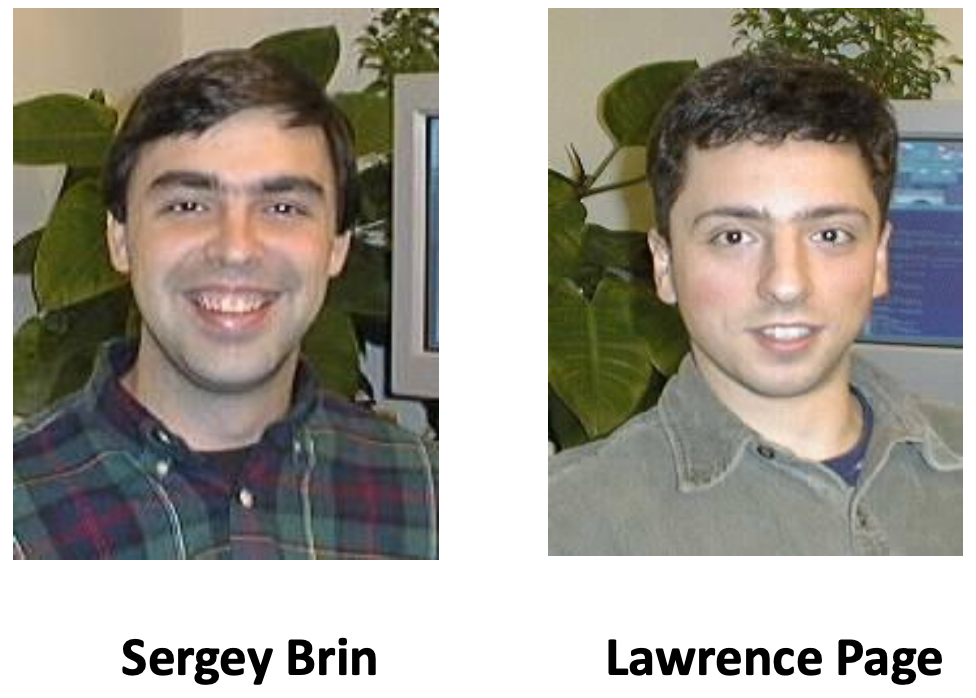
\includegraphics[scale=0.35]{autores.png} 
		\end{minipage}
		
		% Eran ustudiantes de Stanford
		
		% El algoritmo del PageRank se basa en:
		% - las citaciones de documentos académicos.
		% - a pesar del repositorio caótico que es Internet, su contenido heterogénea tiene una estructura.
		
	\end{frame}
	
	%------------------------------------------------
	% La Web como grafo
	\begin{frame}
		
		\frametitle{Premisas del algoritmo PageRank}
		
		Tratar la Web como un grafo dirigido donde:
		
		\vspace{1\baselineskip}
		
		\begin{minipage}{\linewidth}
		\begin{center}
			\begin{tikzpicture}
				% Coloca la imagen en el centro de la página
				\node[inner sep=0pt] (imagen) at (0,0) {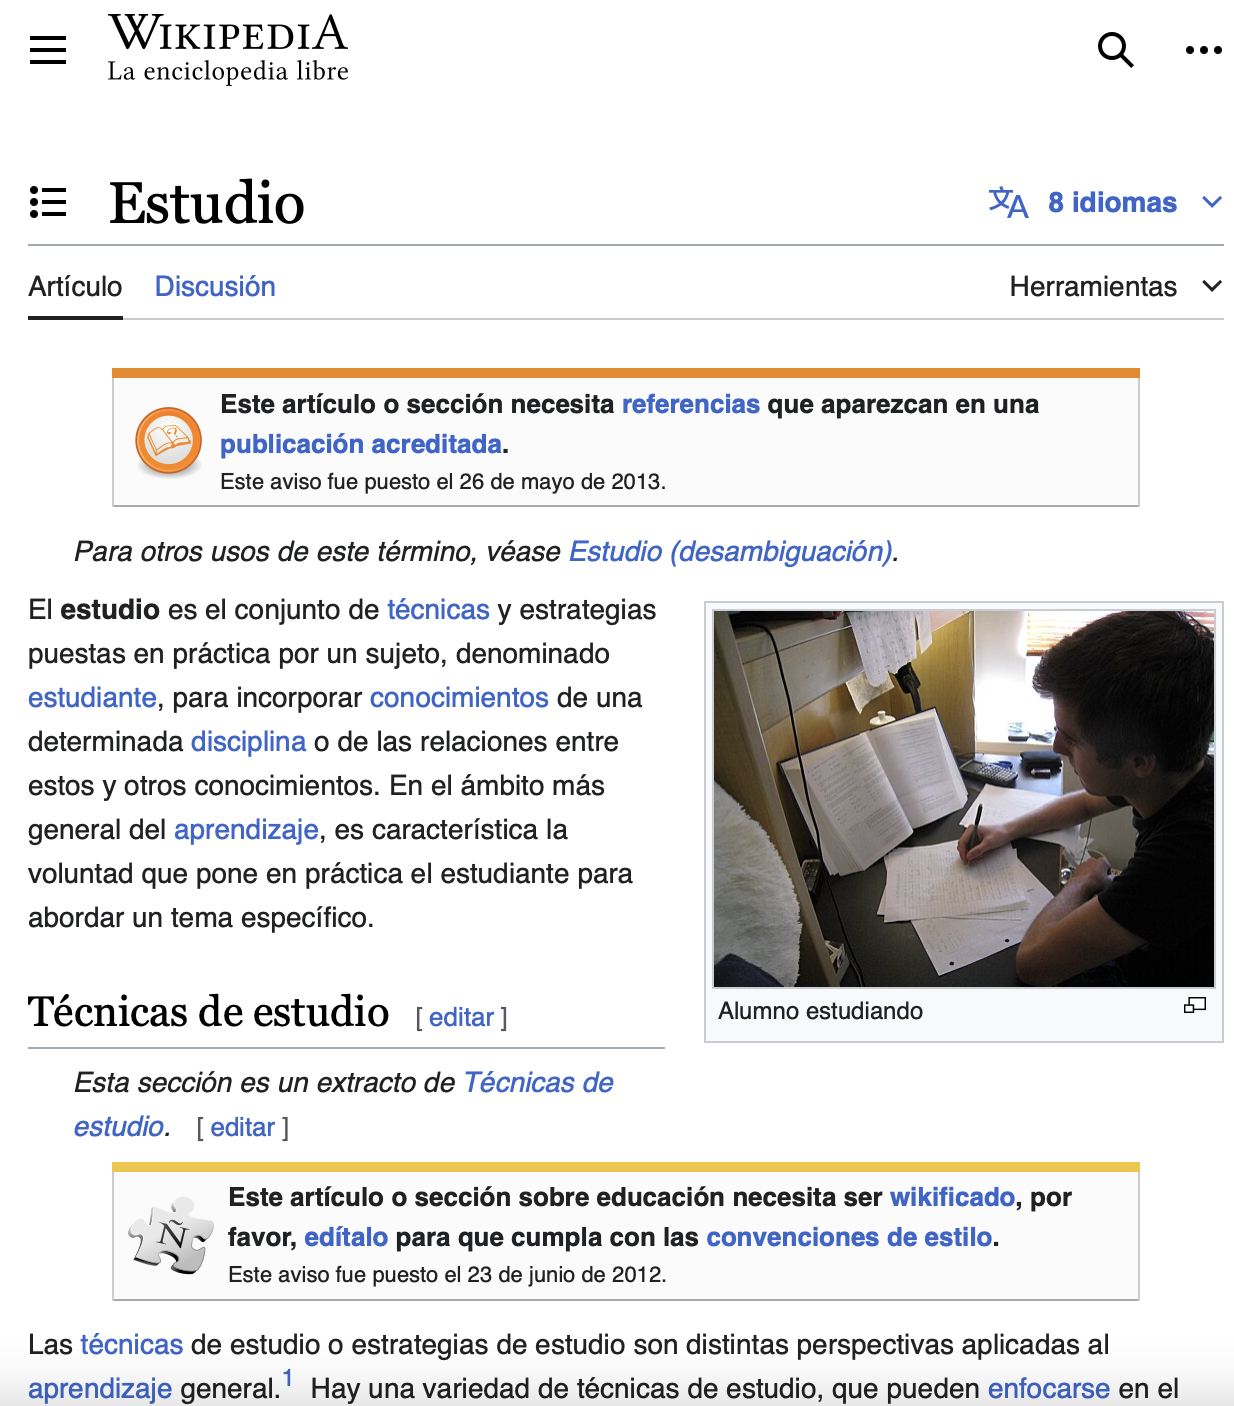
\includegraphics[width=0.35\textwidth]{wikipedia.png}};
				\draw[thick,black] (imagen.south west) rectangle (imagen.north east);
				
				% Fecha 1
				\draw[->, thick] (-2.3,2.1) -- (-3.7,2);
				\node[left,text width=4cm,align=center] at (-3.6,2) {Artículo de Wikipedia (página u otro archivo de la web) $=$ \textbf{Nodo}};
				
				% Flecha 2
				\draw[->, thick] (-0.5,-1.7) -- (-3,-0.7);
				\draw[->, thick] (-1.7,-0.6) -- (-3,-0.6);
				\draw[->, thick] (-0.8,0) -- (-3,-0.5);
				\node[left,text width=4cm,align=center] at (-3,-0.6) {Artículos referenciados (referencias de salida) $=$ \textbf{Aristas de salida}};
				
				% Flecha 3
				\draw[->, thick] (5,1.3) -- (3,2);
				\node[left,text width=4cm,align=center] at (7,0.3) {Existen otros artículos con hipervínculos hacia este (referencias de entrada) $=$ \textbf{Aristas de entrada}};
				
			\end{tikzpicture}
		\end{center}
		\end{minipage}
		
		% La web puede verse como un grafo dirigido interconectado a través de los links. 
		% Un nodo no necesariamente tiene que ser un sitio web, puede ser documentos, imágenes o cualquier tipo de dato alojada en internet y que otros datos la referencien o este referencia al resto.
		
	\end{frame}
	
	%------------------------------------------------
	% Asunciones referentes a la importancia de una página web
	\begin{frame}
		
		\frametitle{Suposiciones referentes a la importancia de una página web}
		
		\begin{itemize}
			\item Un nodo (página web) $A$ con hipervínculos hacia un nodo $B$ le brinda a $B$ una descripción (relevancia) positiva. \\[2mm]
			% Dado un nodo de importancia, todo lo que apunte a él puede ser de interés.
			
			\item El hipervínculo de $A$ a $B$ representa un respaldo de la página $B$ por parte del creador de la página $A$.
			% Este no es siempre el caso; por ejemplo, muchos enlaces entre páginas dentro de un único sitio web provienen del usuario de una plantilla común. Por ejemplo, la mayoría de los sitios web corporativos tienen un puntero desde cada página a una página que contiene un aviso de derechos de autor; esto claramente no es un respaldo. En consecuencia, las implementaciones de algoritmos de análisis de enlaces normalmente descartarán dichos enlaces "internos".
			
		\end{itemize}
		
		% Al analizar la calidad y la cantidad de enlaces a un sitio, determina la importancia de una página.
		
		% Obtener enlaces de sitios web con autoridad es algo realmente bueno. Además, Google considera que el enlace añade credibilidad a tu contenido, y esto evidentemente tiene un impacto positivo en tu posicionamiento web.
		
		% Para “rankear” más alto, necesitas enlaces de sitios web de calidad.
		
		% Por otro lado, esos sitios web, a su vez, necesitan enlaces de otros sitios web de calidad. La puntuación actúa como una medida de la calidad relativa de un sitio web en comparación con otros sitios que el motor de búsqueda podría mostrar.
		
		\vspace{2\baselineskip}
		
		\only<2>{
			\begin{exampleblock}{}
				A diferencia de la recuperación de información en ambientes locales, en la web se utilizan los hipervínculos para definir la relevancia de cada sitio web con respecto a una consulta.
			\end{exampleblock}
			
			\vspace{1\baselineskip}
			Puede considerarse también el uso de las palabras claves asociadas a los hipervínculos para establecer la relevancia. Ejemplo:
			
			\centering
			\texttt{<a href="http://www.acm.org/jacm/" >Journal of the ACM</a>}
			
			% El uso de los términos pueden ser usados para definir relaciones. De igual manera, las referecnias son normalizadas con idf. No obstante, trabajar con estos principios pueden trae consecuencias negativas en los resultados arrojados porque favorece al spam.
		}
		
	\end{frame}
	
	%------------------------------------------------
	% Ideas generales del algoritmo PageRank
	\begin{frame}
		
		\frametitle{Ideas generales del algoritmo PageRank}
		
		\begin{itemize}
			
			\item El algoritmo es la función de ranking para los entornos en la web. \\[2mm]
			
			\item Es una medida de la cantidad y la visibilidad o calidad de los enlaces que recibe una página web.  \\[2mm]
			
			\item Las aristas entrantes se consideran \emph{votos}. \\[2mm]
			
			\item Las aristas provenientes de páginas ``importantes'' o con autoridad tienen mayor peso o valor.
			
		\end{itemize}
		
	\end{frame}
	
	%------------------------------------------------
	% Definición (simplificada) del algoritmo PageRank
	\begin{frame}
		
		\frametitle{Definición de la función PageRank}
		
		$$R(u) = c \sum_{v \in B_u} \frac{R(v)}{N_v}$$ \\[2mm]
		
		\only<1>{
			\begin{itemize}
				\item $u$ : página web 
				\item $R(u)$ : valor del PageRank para $u$
				\item $B_u$ : conjunto de enlaces de entrada (\emph{backlinks}) de la página $u$
				\item $F_u$ : conjunto de enlaces de salida (\emph{forwardlinks}) desde la página $u$
				\item $N_i = |F_i|$
				\item $c$ : factor de normalización 
				% Asegura que el algoritmo converge correctamente.
			\end{itemize}
		}
		
		\only<2>{
			\begin{itemize}
				\vspace{3\baselineskip}
				
				\item El valor de cada página es dividido entre sus enlaces de directos.
				\item El cálculo es recursivo.
				\item Puede computarse comenzando por cualquier nodo e iterar hasta que converja el algoritmo.
			\end{itemize}
		}
		
	\end{frame}
	
	%------------------------------------------------
	% Problema del algoritmo
	\begin{frame}
		
		\frametitle{Problema $\#1$}
		
		Para una cierta red se tiene la siguiente topología: \\[2mm]
		
		\begin{centering}
			
			\begin{tikzpicture}
				% Nodos
				\node[draw, circle, align=center] (nodo1) at (0,0) {Nodo 1 \\ $R(n_1) = 1$};
				\node[draw, circle, align=center] (nodo2) at (4,0) {Nodo 2 \\ $R(n_2) = 1$};
				% Flechas
				\draw[->, thick] (nodo1) to[out=-30, in=-150] (nodo2);
				\draw[->, thick] (nodo2) to[out=150, in=30] (nodo1);
			\end{tikzpicture}
			
		\end{centering}
		
		\vspace{1\baselineskip}
		
		\textcolor{purple}{¿Qué problema puede existir?} 
		
		\only<2->{
			R/: En cada iteración el valor de cada nodo no se modificará porque no hay cambios en su clasificación.
	
			\vspace{1\baselineskip}
			
			Por tanto, es necesario modificar la forma de calcular el valor de cada página web.
		}
	\end{frame}
	
	%------------------------------------------------
	% Problema del algoritmo
	\begin{frame}
		
		\frametitle{Problema $\#2$}
		
		Se tiene el siguiente grafo de la Web: 
		
		\vspace{2\baselineskip}
		
		\begin{minipage}{0.45\textwidth}
			\centering
			
			Inicio \\[2mm]
			
			\begin{tikzpicture}[->,>=stealth',shorten >=1pt,auto,node distance=2cm,thick,main node/.style={circle,draw,font=\small, minimum size=1cm}]
				% Definición de los nodos
				\node[main node] (1) {R(n1)=0.2};
				\node[main node] (2) [above right of=1] {R(n2)=0.2};
				\node[main node] (3) [below right of=2] {R(n3)=0.2};
				\node[main node] (4) [below left of=3] {R(n4)=0.2};
				\node[main node] (5) [below left of=1] {R(n5)=0.2};
				
				% Conexiones cíclicas
				\path[every node]
				(1) edge [bend right] node {} (2)
				(2) edge [bend right] node {} (3)
				(3) edge [bend right] node {} (4)
				(4) edge [bend right] node {} (1);
				
				% Conexión del quinto nodo hacia uno de los nodos cíclicos
				\path[every node]
				(5) edge [bend left] node {} (1);
			\end{tikzpicture}
			
		\end{minipage}%
		\hfill
		\begin{minipage}{0.45\textwidth}
			\centering
			
			Iteración \only<1>{$\#1$}\only<2>{$\#2$}\only<3>{$\#\infty$} \\[2mm]
			
			\begin{tikzpicture}[->,>=stealth',shorten >=1pt,auto,node distance=2cm,thick,main node/.style={circle,draw,font=\small, minimum size=1cm}]
				
				% Definición de los nodos
				\node[main node] (1) {R(n1)=\only<1>{\textcolor{red}{0.4}}\only<2>{\textcolor{red}{0.8}}\only<3>{\textcolor{red}{$+\infty$}}};
				
				\node[main node] (2) [above right of=1] {R(n2)=\only<1>{\textcolor{red}{0.4}}\only<2>{\textcolor{red}{0.8}}\only<3>{\textcolor{red}{$+\infty$}}};
				
				\node[main node] (3) [below right of=2] {R(n3)=\only<1>{\textcolor{red}{0.4}}\only<2>{\textcolor{red}{0.8}}\only<3>{\textcolor{red}{$+\infty$}}};
				
				\node[main node] (4) [below left of=3] {R(n4)=\only<1>{\textcolor{red}{0.4}}\only<2>{\textcolor{red}{0.8}}\only<3>{\textcolor{red}{$+\infty$}}};
				
				\node[main node] (5) [below left of=1] {R(n5)=0.2};
				
				% Conexiones cíclicas
				\path[every node]
				(1) edge [bend right] node {} (2)
				(2) edge [bend right] node {} (3)
				(3) edge [bend right] node {} (4)
				(4) edge [bend right] node {} (1);
				% Conexión del quinto nodo hacia uno de los nodos cíclicos
				\path[every node]
				(5) edge [bend left] node {} (1);
			\end{tikzpicture}
		\end{minipage}%
		
	\end{frame}
	
	%------------------------------------------------
	% Problema del algoritmo
	\begin{frame}
		
		\frametitle{Problema $\#2$: \emph{Rank sink}}
		
		\begin{minipage}{0.45\textwidth}
		
			\only<1>{
				\begin{exampleblock}{\emph{Rank sink}}
					Página web o un conjunto de páginas web que no tienen enlaces salientes o que solo tienen enlaces salientes entre ellas mismas, sin enlaces que apunten hacia otras páginas de la red. 
				\end{exampleblock}
				
				\vspace{2\baselineskip}
				
				El motivo de tomar $c<1$ es evitar el estancamiento del algoritmo, especialmente cuando hayan ciclos.
				% Al reducirlo por debajo de 1, se garantiza que una pequeña fracción de la probabilidad (1-c) se distribuya uniformemente entre todas las páginas web, lo que evita que el PageRank se estanque en "rank sinks". La mayoría de la probabilidad (c) se distribuye según los enlaces entrantes, lo que permite que el PageRank fluya y se distribuya de manera más equitativa en la web.
			}
			
			\only<2->{
				\begin{itemize}
					
					\item La existencia de un lazo provoca que el PageRank no fluya fuera de ese conjunto, conduciendo a una distribución desigual en la Web. \\[1mm]
					% porque las páginas dentro del lazo tienden a acumular PageRank sin redistribuirlo a otras páginas.
					
					\item Afecta la efectividad del algoritmo. \\[1mm]
					
					\item Puede ser provocado por páginas huérfanas (sin enlaces entrantes) o estructuras de enlaces mal diseñadas. \\[2mm]

				\end{itemize}
			}
			
		\end{minipage}%
		\hfill
		\begin{minipage}{0.45\textwidth}
			\centering
			
			\begin{tikzpicture}[->,>=stealth',shorten >=1pt,auto,node distance=2cm,thick,main node/.style={circle,draw,font=\small, minimum size=1cm}]
				
				% Definición de los nodos
				\node[main node] (1) {R(n1)=$\infty$};
				\node[main node] (2) [above right of=1] {R(n2)=$\infty$};
				\node[main node] (3) [below right of=2] {R(n3)=$\infty$};
				\node[main node] (4) [below left of=3] {R(n4)=$\infty$};
				\node[main node] (5) [below left of=1] {R(n5)=2};
				
				% Conexiones cíclicas
				\path[every node]
				(1) edge [bend right] node {} (2)
				(2) edge [bend right] node {} (3)
				(3) edge [bend right] node {} (4)
				(4) edge [bend right] node {} (1);
				% Conexión del quinto nodo hacia uno de los nodos cíclicos
				\path[every node]
				(5) edge [bend left] node {} (1);
			\end{tikzpicture}
			
		\end{minipage}%
		
		
		% Para abordar el problema de los "rank sinks", los motores de búsqueda y los desarrolladores de algoritmos de ranking pueden implementar diversas técnicas, como la introducción de un factor de amortiguación en el cálculo del PageRank o ajustar la manera en que se manejan las páginas huérfanas. Estas técnicas ayudan a garantizar que el PageRank fluya de manera más equitativa y efectiva a través de la web.
		
		\only<3>{
			\vspace{2\baselineskip}
			
			Existe un modo de solucionarlo y es usando Modelos de Paseo Aleatorio.
		}
		
	\end{frame}
	
	%------------------------------------------------
	% Modelos de Paseo Aleatorio
	\begin{frame}
		
		\frametitle{Modelos de Paseo Aleatorio (Random Walker Models, RWM)}
		
		\begin{exampleblock}{}
			Modelo matemático que describe el comportamiento estocástico (aleatorio) de un sistema que evoluciona a lo largo del tiempo y/o espacio.
		\end{exampleblock}
		
		\vspace{2\baselineskip}
		
		Los caminos aleatorios de RWM pueden verse como cadenas específicas en las Cadenas de Markov (Markov Chain) y viceversa.
		
		
	\end{frame}
	
	%------------------------------------------------
	% Refinición (arreglada) del función PageRank
	\begin{frame}
		
		\frametitle{Redefinición de la función PageRank con RWM}
		
		$$R'(u) = c \sum_{v \in B_u} \frac{R'(v)}{N_v} + cE(u)$$ \\[2mm] 
		
		\begin{itemize}
			
			\item Se intenta maximizar $c$ y $||R(u)||_1 = 1$
			% Norma de Manhattan : se define como la suma de los valores absolutos de los elementos del vector o matriz
			
			\item $E(u)$ es un vector asociado a $u$\\
			$E$ puede verse desde la perspectiva de RWM.
			
		\end{itemize}

	\end{frame}
	
	%------------------------------------------------
	% 
	\begin{frame}
		
		\frametitle{Redefinición de la función PageRank}
		
		Una adaptación usada para la función del algoritmo es 
		
		\only<1>{
			$$R(u) = d \sum_{v \in B_u} \frac{R(v)}{N_v} + 1 - d$$
		}
		
		\only<2>{
			\begin{align*}
				R'(u) &= \textcolor{red}{d \sum_{v \in B_u} \frac{R'(v)}{N_v}} + 1 - d \\
				&\text{\vspace{1\baselineskip} Representa el cambio para llegar a} \\
				&\text{\vspace{1\baselineskip} $u$ desde páginas que la apuntan ($B_u$)}
			\end{align*}
		
			\vspace{2\baselineskip}
		}
		
		\only<3>{
			\begin{align*}
				R'(u) &= d \sum_{v \in B_u} \frac{R'(v)}{N_v} + \textcolor{red}{1 - d} \\
				&\begin{aligned}
					&\hspace{2cm}\text{Representa el cambio para llegar a la página  $u$} \\
					&\hspace{2cm}\text{desde cualquier otra página de la red (paseo aleatorio)}
				\end{aligned}
			\end{align*}
			
			\vspace{2\baselineskip}
		}
		
		donde:
		\begin{itemize}
			\item $d=0.85$ usualmente
			\item $N$ : total de páginas web en la red 
		\end{itemize}	

		\centering
		\vspace{1.5\baselineskip}
		{\scriptsize Consultar ``Brin, Sergey;Page, Lawrence. The anatomyof a large-scale hypertextual Web search engine. 1998'' \url{https://snap.stanford.edu/class/cs224w-readings/Brin98Anatomy.pdf}}

	\end{frame}
	
	%------------------------------------------------
	% Criterios de convergencia
	\begin{frame}
		
		\frametitle{Criterios de convergencia del algoritmo de PageRank}
		
		
		\begin{itemize}
			
			\item Cambio en los valores 
			% Se puede monitorear el cambio en los valores de PageRank entre iteraciones sucesivas. Si los cambios son menores que un umbral predefinido o si los valores de PageRank se estabilizan, se considera que el algoritmo ha convergido.
			
			\item Norma de la diferencia entre vectores 
			% Se puede calcular la norma (o magnitud) de la diferencia entre los vectores de PageRank en dos iteraciones consecutivas. Si la norma es menor que un cierto umbral, se considera que el algoritmo ha convergido.
			
			\item Número máximo de iteraciones
			% Se puede establecer un número máximo de iteraciones para el algoritmo. Si se alcanza este límite sin que se satisfagan otros criterios de convergencia, el algoritmo se detiene y se considera que ha convergido, aunque esto puede no ser garantía de convergencia total.
			
		\end{itemize}
		
		\pause
		\vspace{2\baselineskip}
		
		Recuerde que: 
		\begin{itemize}
			\item La constante $c\ (d)$ ayuda a la convergencia del método.
			
			\item La convergencia puede depender de
			\begin{itemize}
				\item la estructura de la red de los enlaces,
				\item la distribución inicial de PageRank,
				\item la tolerancia de convergencia establecido y 
				\item el método de cálculo utilizado.
			\end{itemize}
			
		\end{itemize}
		
	\end{frame}
	
	%------------------------------------------------
	% Break
	{
		\setbeamertemplate{background canvas}
		{%
			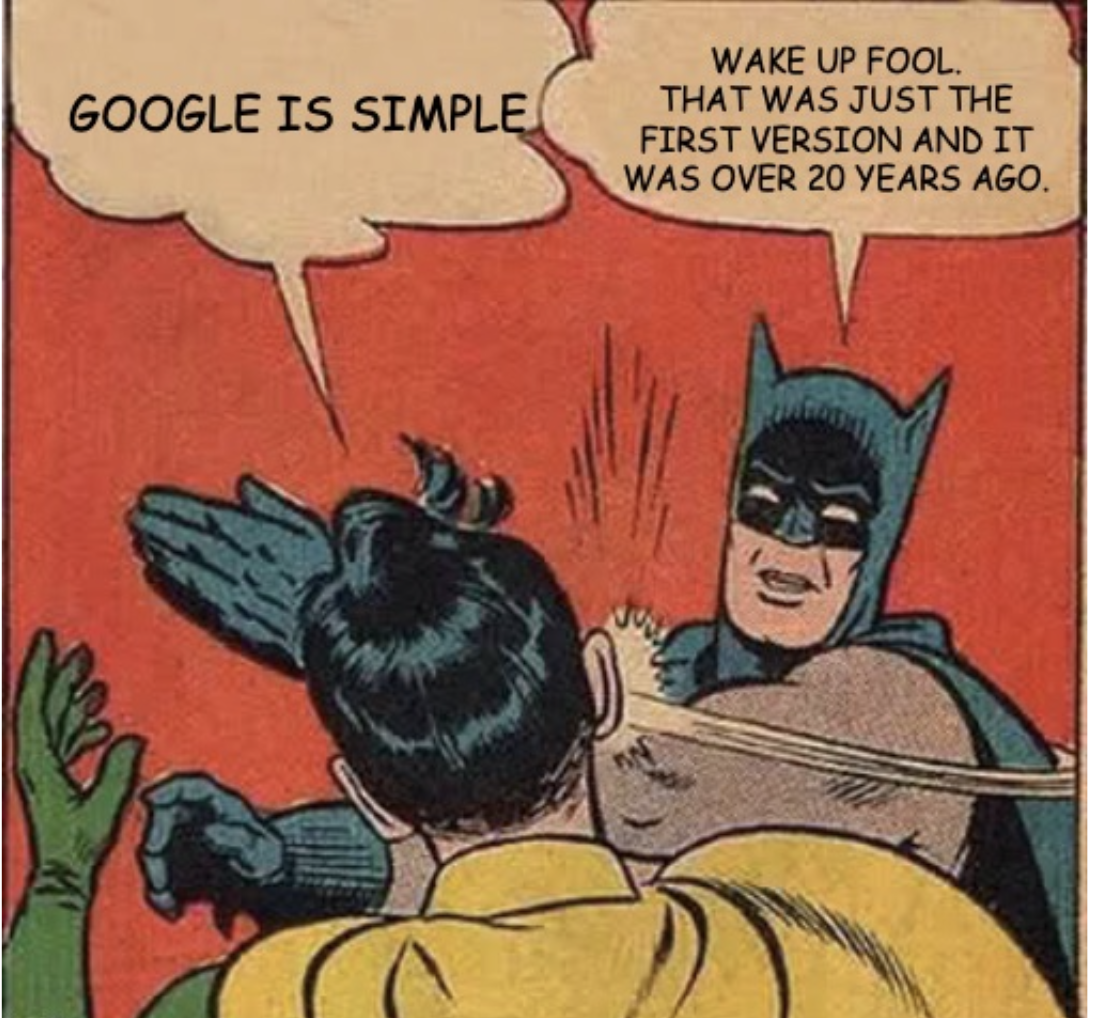
\includegraphics[width=\paperwidth,height=\paperheight]{meme.png}
		}
		
		% De la publicación del paper hasta el 2023, han existido alrededor de 21 actualizaciones.
		
		\begin{frame}
		\end{frame}
	}
	
	%------------------------------------------------
	% Otro algoritmo de enlaces
	\begin{frame}
		
		\frametitle{¿PageRank es el único algoritmo de enlaces?}
		
		% Otro algoritmo para evaluar la importancia y la relevancia de las páginas web en función de los enlaces que reciben de otras páginas es HITS
		
		\begin{alertblock}{Selección de temas inducida por hipertexto (Hypertext Induced Topic Selection, HITS)}
			HITS es un algoritmo de enlaces que no se basa únicamente en la cantidad de enlaces, sino que también considera la calidad de los enlaces. HITS identifica dos tipos de páginas: las autoridades, que tienen muchos enlaces entrantes; y los hubs, que enlazan a muchas autoridades.
		\end{alertblock}
		
		% Autoridades (Authorities): Son páginas web que proporcionan contenido de alta calidad y relevancia en un tema particular. Las autoridades a menudo son identificadas por la cantidad y la calidad de los enlaces entrantes que reciben de otras páginas.
		
		% Hubs: Son páginas web que actúan como directorios o índices, proporcionando enlaces a una variedad de recursos relacionados con un tema específico. Los hubs suelen enlazar a numerosas autoridades y proporcionar una guía para encontrar información sobre un tema determinado.
		
		\vspace{2\baselineskip}
		
		Es utilizado fundamentalmente para comprender y analizar la estructura de los enlaces de la web.
		
	\end{frame}
	
	%------------------------------------------------
	% Posicionamiento en la Web
	\begin{frame}
		
		\frametitle{Tipos de posicionamiento en la Web}
		
		\only<1>{
			\textcolor{purple}{¿Cómo se ordena o se posiciona los resultados de las búsquedas en la Web?} 
		}
		
		\only<2>{
			
				\begin{itemize}
				
				\item Orgánico \\
				Se centra en la clasificación natural de un sitio web en los resultados de búsqueda basada en la relevancia y la autoridad del contenido. \\[1.5mm]
				% Para lograr un buen posicionamiento orgánico, es importante optimizar el contenido del sitio web para las palabras clave relevantes, mejorar la estructura del sitio y obtener enlaces de calidad de otros sitios web.
				
				\item Local \\
				Se centra en mejorar la visibilidad de un negocio en las búsquedas locales. \\[1.5mm]
				% Para mejorar el posicionamiento local, es esencial tener una ficha de Google My Business completa y precisa, obtener reseñas positivas de los clientes y asegurarse de que la información de contacto y la ubicación del negocio sean consistentes en todas las plataformas en línea.
				
				\item Pagado \\
				Implica pagar a los motores de búsqueda por mostrar anuncios relevantes en las páginas de resultados de búsqueda. \\[1.5mm]
				% Esta estrategia generalmente involucra la compra de palabras clave específicas a través de plataformas publicitarias como Google Ads y Bing Ads, y la optimización de la estructura y el contenido de los anuncios para mejorar su relevancia y tasa de clics.
				
				\item En fragmentos destacados \\
				Son fragmentos de contenido que el motor de búsqueda selecciona de una página web y muestra para responder a las consultas de los usuarios de manera rápida y concisa. 
				% Para mejorar las posibilidades de aparecer en fragmentos destacados, es útil proporcionar respuestas claras y concisas a preguntas comunes, usar encabezados descriptivos y estructurar el contenido de manera que sea fácil de entender para los motores de búsqueda.
				
			\end{itemize}
			
			\vspace{2\baselineskip}
			
			La posición de los resultados influye positiva o negativamente a la visibilidad de los sitios web.
			
		}
		
	\end{frame}
	
	%------------------------------------------------
	% Otros aspectos que influyen en el ranking
	\begin{frame}
		
		\frametitle{Otros aspectos que influyen en el ranking}
		
		\begin{itemize}
			\item Relevancia de las palabras en el contexto general
			\item Ubicación de las palabras en el cuerpo de la página web
		\end{itemize}
		
		% \pause
		\vspace{3\baselineskip}
		Responsabilidad de la \textbf{optimización para motores de búsqueda}.
		
	\end{frame}
	
	%------------------------------------------------
	% SEO
	\begin{frame}
		
		\frametitle{Optimización para motores de búsqueda}
		
		\begin{alertblock}{Optimización para motores de búsqueda (Search Engine Optimization, SEO)}
			Serie de técnicas, disciplinas y estrategias de optimización que se implementan en las páginas de un sitio web o blog para mejorar su posicionamiento en los buscadores. Puede entenderse como estrategias de marketing.
		\end{alertblock}
		
		\vspace{2\baselineskip}
		
		Se identifica con el posicionamiento orgánico.
		
	\end{frame}
	
	%------------------------------------------------
	% Técnicas de SEO
	\begin{frame}
		
		\frametitle{Técnicas de SEO}
		
		\begin{itemize}
			\item Optimización del contenido \\[2mm]
			% Crear contenido relevante, útil y de alta calidad que responda a las preguntas y necesidades de los usuarios.
			
			\item Palabras clave \\[2mm]
			% Identificar y utilizar palabras clave relevantes en el contenido y las etiquetas HTML para que los motores de búsqueda puedan entender de qué trata el sitio web.
			
			\item Optimización técnica \\[2mm]
			% Asegurarse de que el sitio web esté bien estructurado, tenga tiempos de carga rápidos, sea compatible con dispositivos móviles y esté libre de errores técnicos que puedan obstaculizar la indexación por parte de los motores de búsqueda.
			
			\item Construcción de enlaces \\[2mm]
			% Obtener enlaces de calidad de otros sitios web relevantes y de autoridad para aumentar la credibilidad y la autoridad del sitio web en los ojos de los motores de búsqueda.
			
			\item Experiencia del usuario
			% Mejorar la experiencia del usuario en el sitio web mediante la navegación fácil, el diseño atractivo y el contenido bien organizado.
			
		\end{itemize}
		
		% El uso estas técnicas en los inicio se ``burlaban'' del algoritmo de posicionamiento en la Web.
		
	\end{frame}
	
	%------------------------------------------------
	% Break
	{
		\setbeamertemplate{background canvas}
		{%
			
\includegraphics[width=\paperwidth,height=\paperheight]{meme2.jpg}
		}
		
		\begin{frame}
		\end{frame}
	}
	
	%------------------------------------------------
	% Ranking del tráfico 
	\begin{frame}
		
		\frametitle{Ranking del tráfico}
		
		\only<1>{
			
			\begin{itemize}
				\item Cantidad de visitantes que recibe un sitio web
				\item Cantidad de páginas vistas dentro de un sitio web
			\end{itemize}
			
			\vspace{2\baselineskip}
			
			Existen sitios web que evalúan el ranking. Las fotos siguientes es la información obtenida de \url{https://www.semrush.com/website/} analizando el sitio oficial de la Universidad de La Habana (\url{uh.cu}). 
		
		}
		
		\only<2>{
				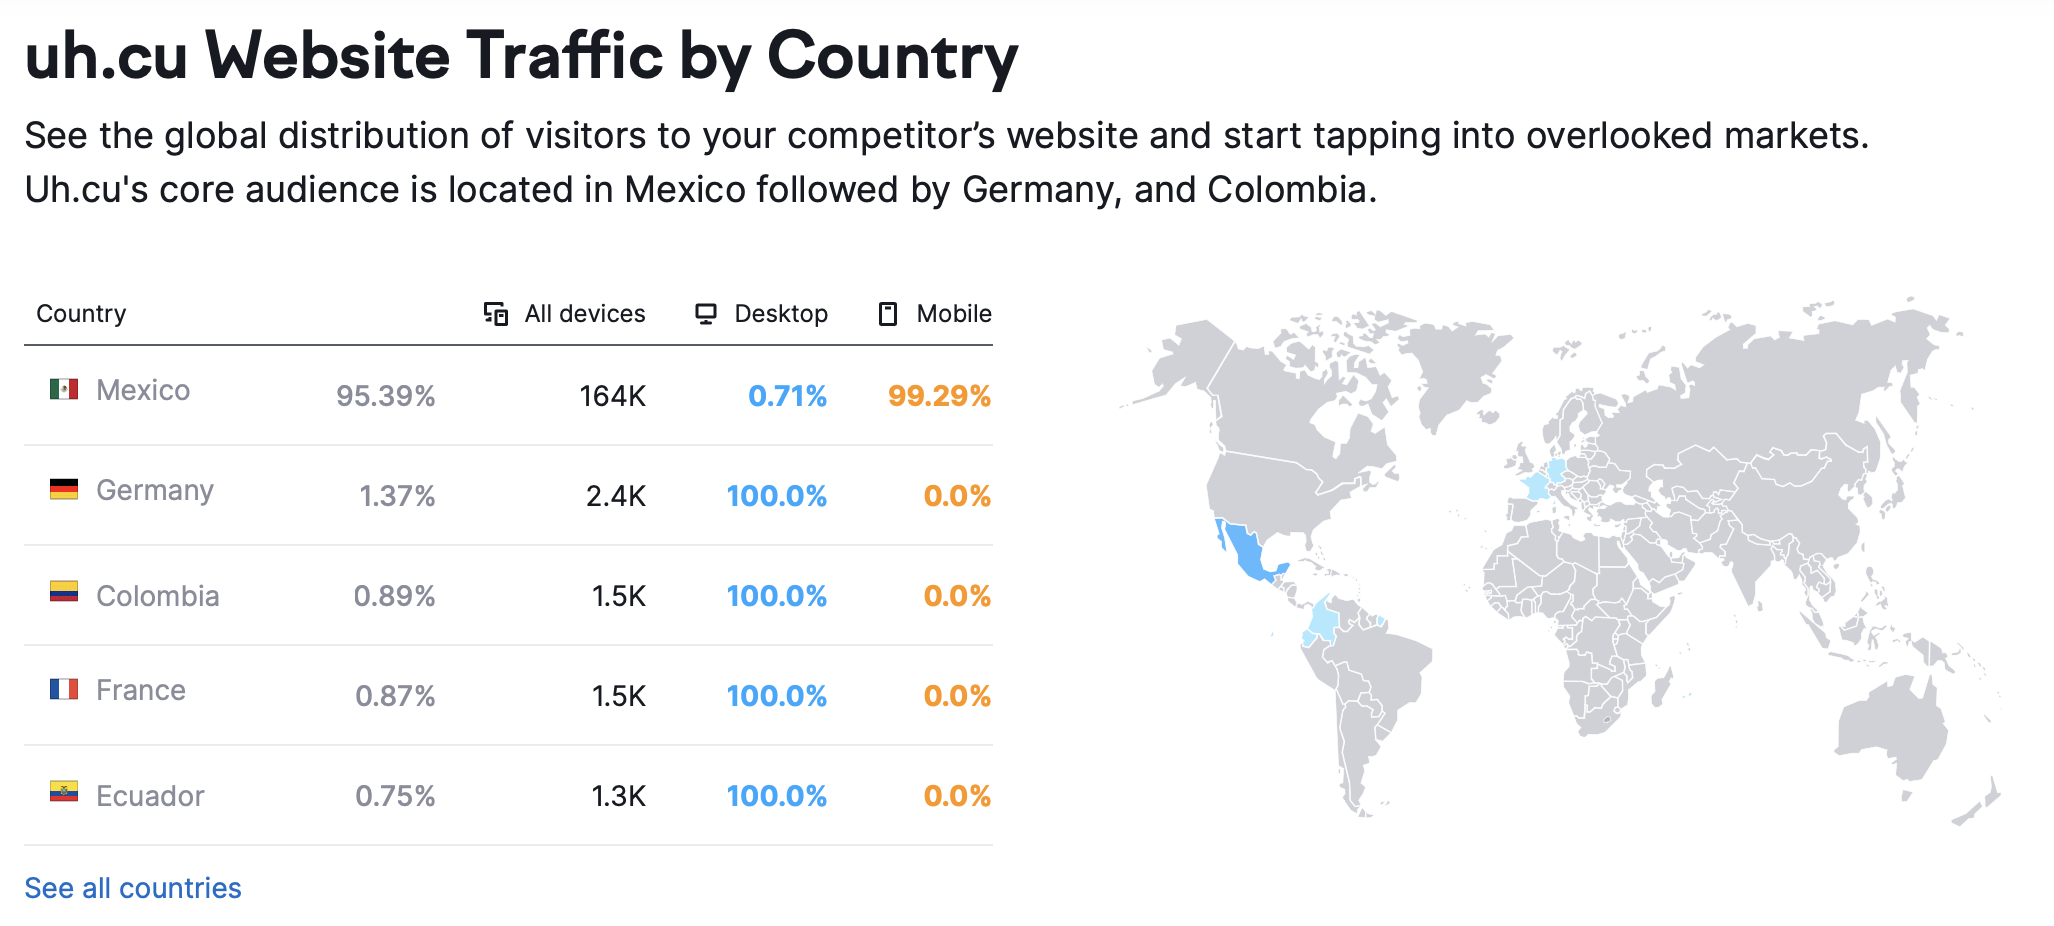
\includegraphics[width=\textwidth]{trafico1.png}
		}
		
		\only<3>{
			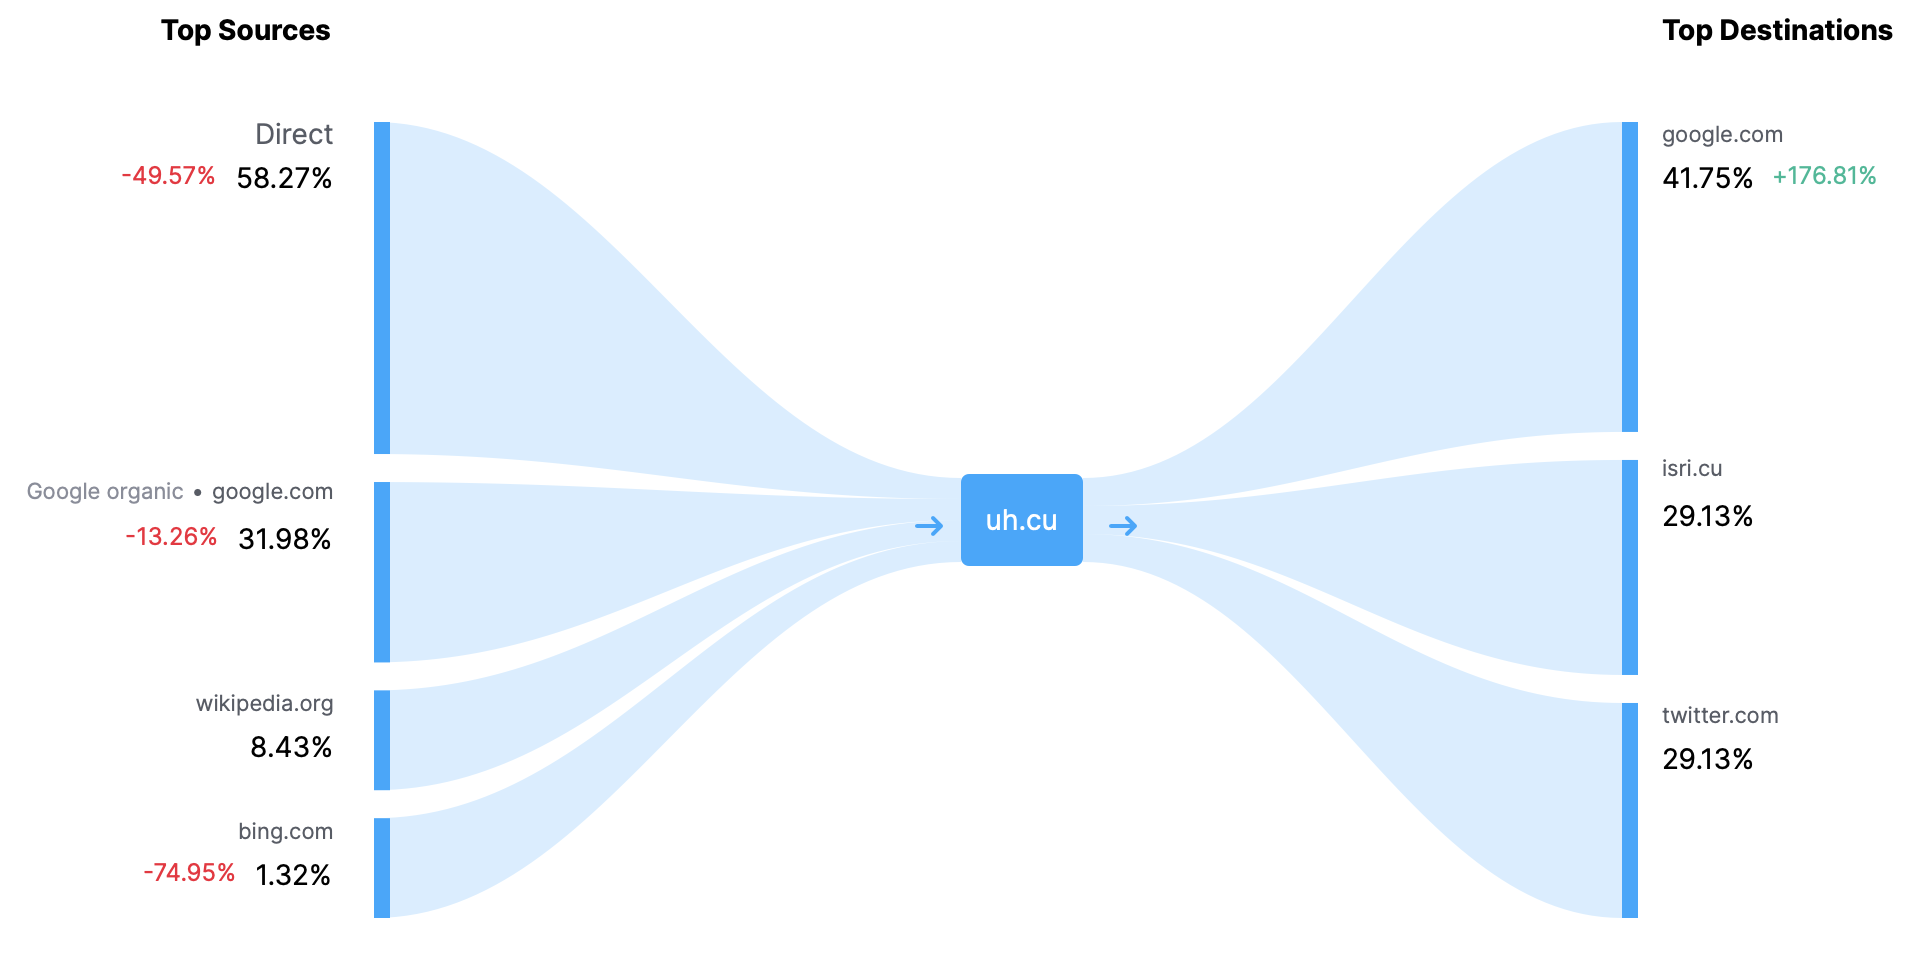
\includegraphics[width=\textwidth]{trafico2.png}
		}
	
	\end{frame}
	
	%------------------------------------------------
	% Conclusiones
	\begin{frame}
		
		\frametitle{Conclusiones}
		
		\begin{itemize}
			
			\item Aumentar la visibilidad de una página web que ocupe los primeros lugares de la lista que devuelven los buscadores ante determinada consulta es objetivo de los algoritmos de enlaces. \\[2mm]
			
			\item PageRank es un algoritmo que ha logrado posicionar a Google como uno de los buscadores favoritos de los usuarios. \\[2mm]
			
			\item La Optimización de Motores de Búsqueda se encuentra en continuas transformaciones para adaptarse a los cambios de la Web y los usuarios.
			
		\end{itemize}
		
	\end{frame}

	%------------------------------------------------
	% Bibliografía
	\begin{frame}
		
		\frametitle{Bibliografía}
		
		\begin{itemize}
						
			\item Page, L., Brin, S., ”The PageRank Citation Ranking: Bringing Order to the Web”. Séptima Conferencia Internacional sobre la World Wide Web (WWW98) en Brisbane, Australia, 1998
			
			\item Manning, Christopher D.;  Raghavan, Prabhakar; Schütze, Hinrich (2007). An Introduction to Information Retrieval. Capítulo 21.
			
		\end{itemize}
		
	\end{frame}
	
	%------------------------------------------------
	% Fin
	\begin{frame}
		\titlepage
	\end{frame}
	
	
	
\end{document} 